%!TEX root = ../report.tex

\section{Technical non-functional requirements}
This section describes the technical aspects that are important to the system as requirements. These requirements determine various APIs and programs that the system will rely on.

% In this section, the technical non-functional requirements important to this system are discussed.

\subsection{Reliability}
% The response time should be about NUMBER mS
% Failure rate ?
% Data transmission
% The margin of error tolerated has to be as low as possible .\\ GK: Margin of error in what aspect?
\begin{longtable}{L{0.1\textwidth} L{0.12\textwidth} L{0.7\textwidth}}
	\textbf{Nr.} & \textbf{Prio}  & \textbf{Description} \\
	\reqRow{rel}{1}{Must}{Sensor sites are equipped with at least two sensors}
	\reqRow{rel}{2}{Must}{Data from the sensors is sent via a TCP connection} % Already mention REST here?
	\reqRow{rel}{3}{Must}{Redundancy} % GK: if redundancy is required, which it should be, in what way?
	%This means adding redundancy to the system so that failure of a component does not mean failure of the entire system
	\bottomrule
\end{longtable}

\subsection{Resilience}
The system needs to be resilient to recover from errors and mistakes without impacting the systems functionality.
\begin{longtable}{L{0.1\textwidth} L{0.12\textwidth} L{0.7\textwidth}}
	\textbf{Nr.} & \textbf{Prio}  & \textbf{Description} \\
	\reqRow{res}{1}{Must}{The system recognizes failures within half an hour}
	\reqRow{res}{2}{Must}{The system recovers from failures without the \qos or the functionality of the system being affected.} % GK: split in two requirements. reduce to detect sensor failures within half an hour
	\reqRow{res}{3}{Must}{The system continues to function with the same \qos in a situation where up to 10\% of the sensors suffer from failures.} % 
	\bottomrule
\end{longtable}

\subsection{Performance}
\begin{longtable}{L{0.1\textwidth} L{0.12\textwidth} L{0.7\textwidth}}
	\textbf{Nr.} & \textbf{Prio}  & \textbf{Description} \\
	\reqRow{perf}{1}{Must}{Data is transmitted from and to the system with a minimum speed of 10 megabits per second} % How to calculate GK: Doesn't really matter for requirements, but good to think about. Also: response time to what? Request? Detecting floods? Furthermore, 10 (just saying something) GB of data is not transferable witihin 1 second if you include connection setup time etc etc
	% GK: only about datatransmission express in dataspeed
	
	\reqRow{perf}{2}{Must}{	The data transmission between the sensors and the system is about 10 mB/sec}
	% How many data the system can receive in one second ?
	\reqRow{perf}{3}{Must}{	The time for the system to calculate if there is a flood or no according to a critical level and the data received from the sensors is about one minute(?). }
	\reqRow{perf}{4}{Must}{	The system should be 99.9 available. }
	\bottomrule
\end{longtable}
% GK: requirement for amount of concurrent users

%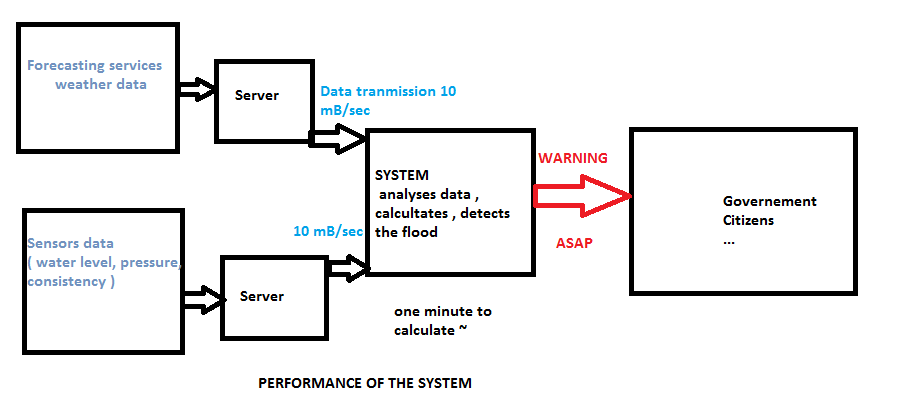
\includegraphics[scale=0.7]{3-requirements/Images/Performance.jpg}

\subsection{Interoperability}
% The system has dependencies on third-party systems. For example, to make predictions about the development of waterlevel, the system will need to retrieve information from water forecasting services. Not only for input, but also for output, the system will need to interoperate with third-party systems. If the system has registered a risk of a flood, it should interact with systems of emergency services and other authorities to alert them and sent relevant information.

\begin{longtable}{L{0.1\textwidth} L{0.12\textwidth} L{0.7\textwidth}}
	\textbf{Nr.} & \textbf{Prio}  & \textbf{Description} \\
	\reqRow{intr}{1}{Must}{The system pulls weather forecasts from five weather forecasting services.}
	\reqRow{intr}{2}{Must}{The system pulls water forecasts from one water forecasting service.}
	\reqRow{intr}{3}{Must}{When the system detects a high risk of flood, it warns the government automatically using the government provided API.}
	\reqRow{intr}{4}{Must}{When the system detects a flood, it automatically tells emergency services where a flood is happening using the API provided by the emergency services.} % GK: change it guidance for emergency service
	\reqRow{intr}{5}{Must}{The system sends out a SMS to all users who are subscribed to flood warnings.}
	\reqRow{intr}{6}{Must}{The systems is able to easily connect to different sensors.}
	% GK: introduce requirement to connect with telecom provider

	\bottomrule
\end{longtable}
\todo[inline]{intr-6 Not measurable}
% GK; Requirement about working with different kind of sensors for the same data

\subsection{Security}
\begin{longtable}{L{0.1\textwidth} L{0.12\textwidth} L{0.7\textwidth}}
	\textbf{Nr.} & \textbf{Prio}  & \textbf{Description} \\
	\reqRow{sec}{1}{Must}{Access to the system is restricted to user accounts that are stored in a database.}
	\reqRow{sec}{2}{Must}{All communication to, from and within the system are encrypted.}
	\reqRow{sec}{3}{Must}{User account information are hashed using bcrypt after being salted with 128 randomly generated characters.}
	\reqRow{sec}{4}{Must}{The system is protected by a firewall that at least scans at the application layer, while also scanning for and preventing DDoS attacks.}
	% WM: does communication within the system mean between the different components of the system?
	\reqRow{sec}{5}{Must}{The system communicates with it's sensors via a REST API that only allows for HTTPS connection.} % Do we want to communicate with the sensors via REST? WM: Could this be more generic? Like: 'the system communicates with the sensors via a secure connection'
	\reqRow{sec}{6}{Must}{All system data must be backed up every 24 hours.}
	\reqRow{sec}{7}{Must}{Backup copies are stored in a secure location which is not in the same area as the system (50 km).} % WM: maybe make area more specific, like range of 50 km or something

	\bottomrule
\end{longtable}
% TODO: how to measure?

\subsection{Scalability}
% The system will be able to cover more areas and use more sensors in the future. GK: too vague, but added scale-3 based on this idea
\begin{longtable}{L{0.1\textwidth} L{0.12\textwidth} L{0.7\textwidth}}
	\textbf{Nr.} & \textbf{Prio}  & \textbf{Description} \\
	\reqRow{scale}{1}{Must}{The database and services run in parallel on a private cloud that is hosted within the Netherlands} % do we want a private cloud? WM: I think public cloud is more scalable (but does government allow it)?
	\reqRow{scale}{2}{Must}{Cassandra is used as database for the storage of the sensor data} % do we want to use cassandra?
	\reqRow{scale}{3}{Must}{The system is configurable to run in different areas and with different sensors.}
	\bottomrule
\end{longtable}
% The system will be developed with more sensors and in more places.
%New functionalities, for example GPS
% ============================================================
% From Gerrit:
% The three main requirements:
% 1: Monitoring activities: the system should monitor activities and properties of
% rivers, waterways, dykes, such as the water level and pressure or the consistency
% of the dyke. Monitoring can be performed through different devices, e.g. analog
% and digital sensors, Unmanned Aerial Vehicles (UAVs) and Vehicular Ad-hoc
% Networks (VANETs) etc.
% 2: Warning: in case of an imminent flood, the system should issue warnings to the
% authorities and emergency services, but also directly to citizens who are
% subscribed for such messages (e.g. through SMS or mobile apps).
% 3: Guidance: the system should provide runtime information to guide its
% constituents or third parties, .e.g. the UAVs may provide information to
% VANETs embedded in vehicles crossing the area, thereby guiding vehicles
% driving towards a flood area to avoid certain routes. Meanwhile, the VANETs
% can also provide an alternative route to emergency services or citizens to avoid
% the flood area. 
% ToDo:
% Stakeholders
% Use-cases
% Make them smart
% Assign value (must/should/...
% ============================================================